\documentclass[11pt]{article}

\usepackage[letterpaper,margin=0.9in]{geometry}
\usepackage[utf8]{inputenc}
\usepackage{xcolor}
\definecolor{MidnightBlue}{HTML}{12233F}
\definecolor{RadarBlue}{HTML}{2563EB}
\definecolor{RadarInk}{HTML}{243247}
\definecolor{RadarMuted}{HTML}{5C6B80}
\definecolor{RadarRule}{HTML}{D7DFEA}
\definecolor{RadarSky}{HTML}{EAF1FF}
\definecolor{LinkRed}{HTML}{CC0000}
\definecolor{CiteBlue}{HTML}{0000CC}
\usepackage{graphicx}
\usepackage{pgf}
\usepackage{array}
\usepackage{booktabs}
\usepackage{tabularx}
\usepackage{longtable}
\usepackage[numbers,sort&compress]{natbib}
\usepackage[hypcap=false]{caption}
\usepackage{hyperref}

\hypersetup{
  colorlinks=true,
  linkcolor=LinkRed,
  urlcolor=CiteBlue,
  citecolor=CiteBlue,
  pdftitle={Benchmark RADAR: Living Search Engine for Retrieval and Discovery of AI Benchmark Research},
  pdfauthor={Koutian Wu and Junjie Zhou}
}

\setlength{\parindent}{1.2em}
\setlength{\parskip}{0.25em}
\setlength{\tabcolsep}{4pt}
\renewcommand{\arraystretch}{1.15}
\sloppy

\newcolumntype{Y}{>{\raggedright\arraybackslash}X}
\newcolumntype{L}[1]{>{\raggedright\arraybackslash}p{#1}}
\newcommand{\reportversion}{v0.10.0}
% Generated by scripts/export_report_figure_data.py; do not hand-edit.
% Dated figure inputs, not a second source of manuscript prose.
% site/data/benchmark-index.json SHA-256: b8d10892e25fe0fe63856f31e1645b41ee7d0f277fedaf308bd8f707852dbff2
% site/data/radar.json SHA-256: 83e33bd88be7639b2876e33c3c1fa18a1980b06ff721ee10cf8cf0d923bef703
\newcommand{\ReportDataCutoff}{2026-09-06}
\newcommand{\ReportObservationCount}{10702}
\newcommand{\ReportArtifactCount}{6304}
\newcommand{\ReportSnapshotCount}{45}
\newcommand{\ReportCatalogCount}{1283}
\newcommand{\ReportCatalogSourceCount}{4}
\newcommand{\ReportLLMStatsCount}{687}
\newcommand{\ReportOpenCompassCount}{461}
\newcommand{\ReportArtificialAnalysisCount}{25}
\newcommand{\ReportModelReportCount}{110}
\newcommand{\ReportSourceMaximum}{3394}
\newcommand{\ReportSourceBars}{%
  \SourceBar{0}{Hugging Face}{3394}%
  \SourceBar{1}{GitHub}{2423}%
  \SourceBar{2}{arXiv}{1899}%
  \SourceBar{3}{Semantic Scholar}{1039}%
  \SourceBar{4}{OpenAlex}{777}%
  \SourceBar{5}{8 other labels}{1170}%
}

\newcommand{\ReportNumber}[1]{\pgfmathprintnumber[fixed,precision=0,1000 sep={,},assume math mode=true]{#1}}
\newcommand{\datacutoff}{\ReportDataCutoff}
\newcommand{\gitcommit}{76a6180}
\graphicspath{{figures/}}

\title{\textbf{Benchmark RADAR: Living Search Engine for Retrieval and Discovery of AI Benchmark Research}}
\author{Koutian Wu$^{1,2}$ \footnote{\small $^*$Corresponding author: \href{mailto:k@tacite.ai}{k@tacite.ai}} \quad Junjie Zhou$^4$ \quad Ergan Shang$^3$ \quad Jiayu Wang $^5$ \quad Pengqian Han$^6$\\[0.35em]
\small $^1$ Earth and Space AI \quad
\small $^2$ Tacite AI \quad
\small $^3$ Carnegie Mellon University\\
\small $^4$ Hangzhou Dianzi University
\small $^5$ Xi'an Jiaotong University\\
\small $^6$ The University of Auckland
}
\date{}

\begin{document}
\maketitle
\vspace{-2.0em}
\begin{abstract}
Benchmark researchers and model developers need to find relevant evaluations, trace their sources, and determine which reported scores can be compared. Benchmark Radar collects benchmark papers, repositories, datasets, catalog entries, and model reports in a searchable system. It records which benchmarks model reports mention and preserves the evaluation settings attached to numeric scores. As of \datacutoff{}, the collection contained \ReportNumber{\ReportObservationCount} source observations, meaning records collected from public sources, and \ReportNumber{\ReportArtifactCount} artifacts after observations with matching identifiers were grouped. Its catalog held \ReportNumber{\ReportCatalogCount} searchable benchmark records. Model reports mentioned 110 benchmarks and supplied 322 scores across 86 benchmark tracks, each collecting results for a named benchmark. The web dashboard, RSS feed, JSON downloads, and local search clients provide access to this evidence. We describe the collection and search methods, examine source coverage and benchmark adoption, and assess the limits of score comparisons when evaluation settings differ.
\end{abstract}

\begin{center}
\vspace{0.3em}
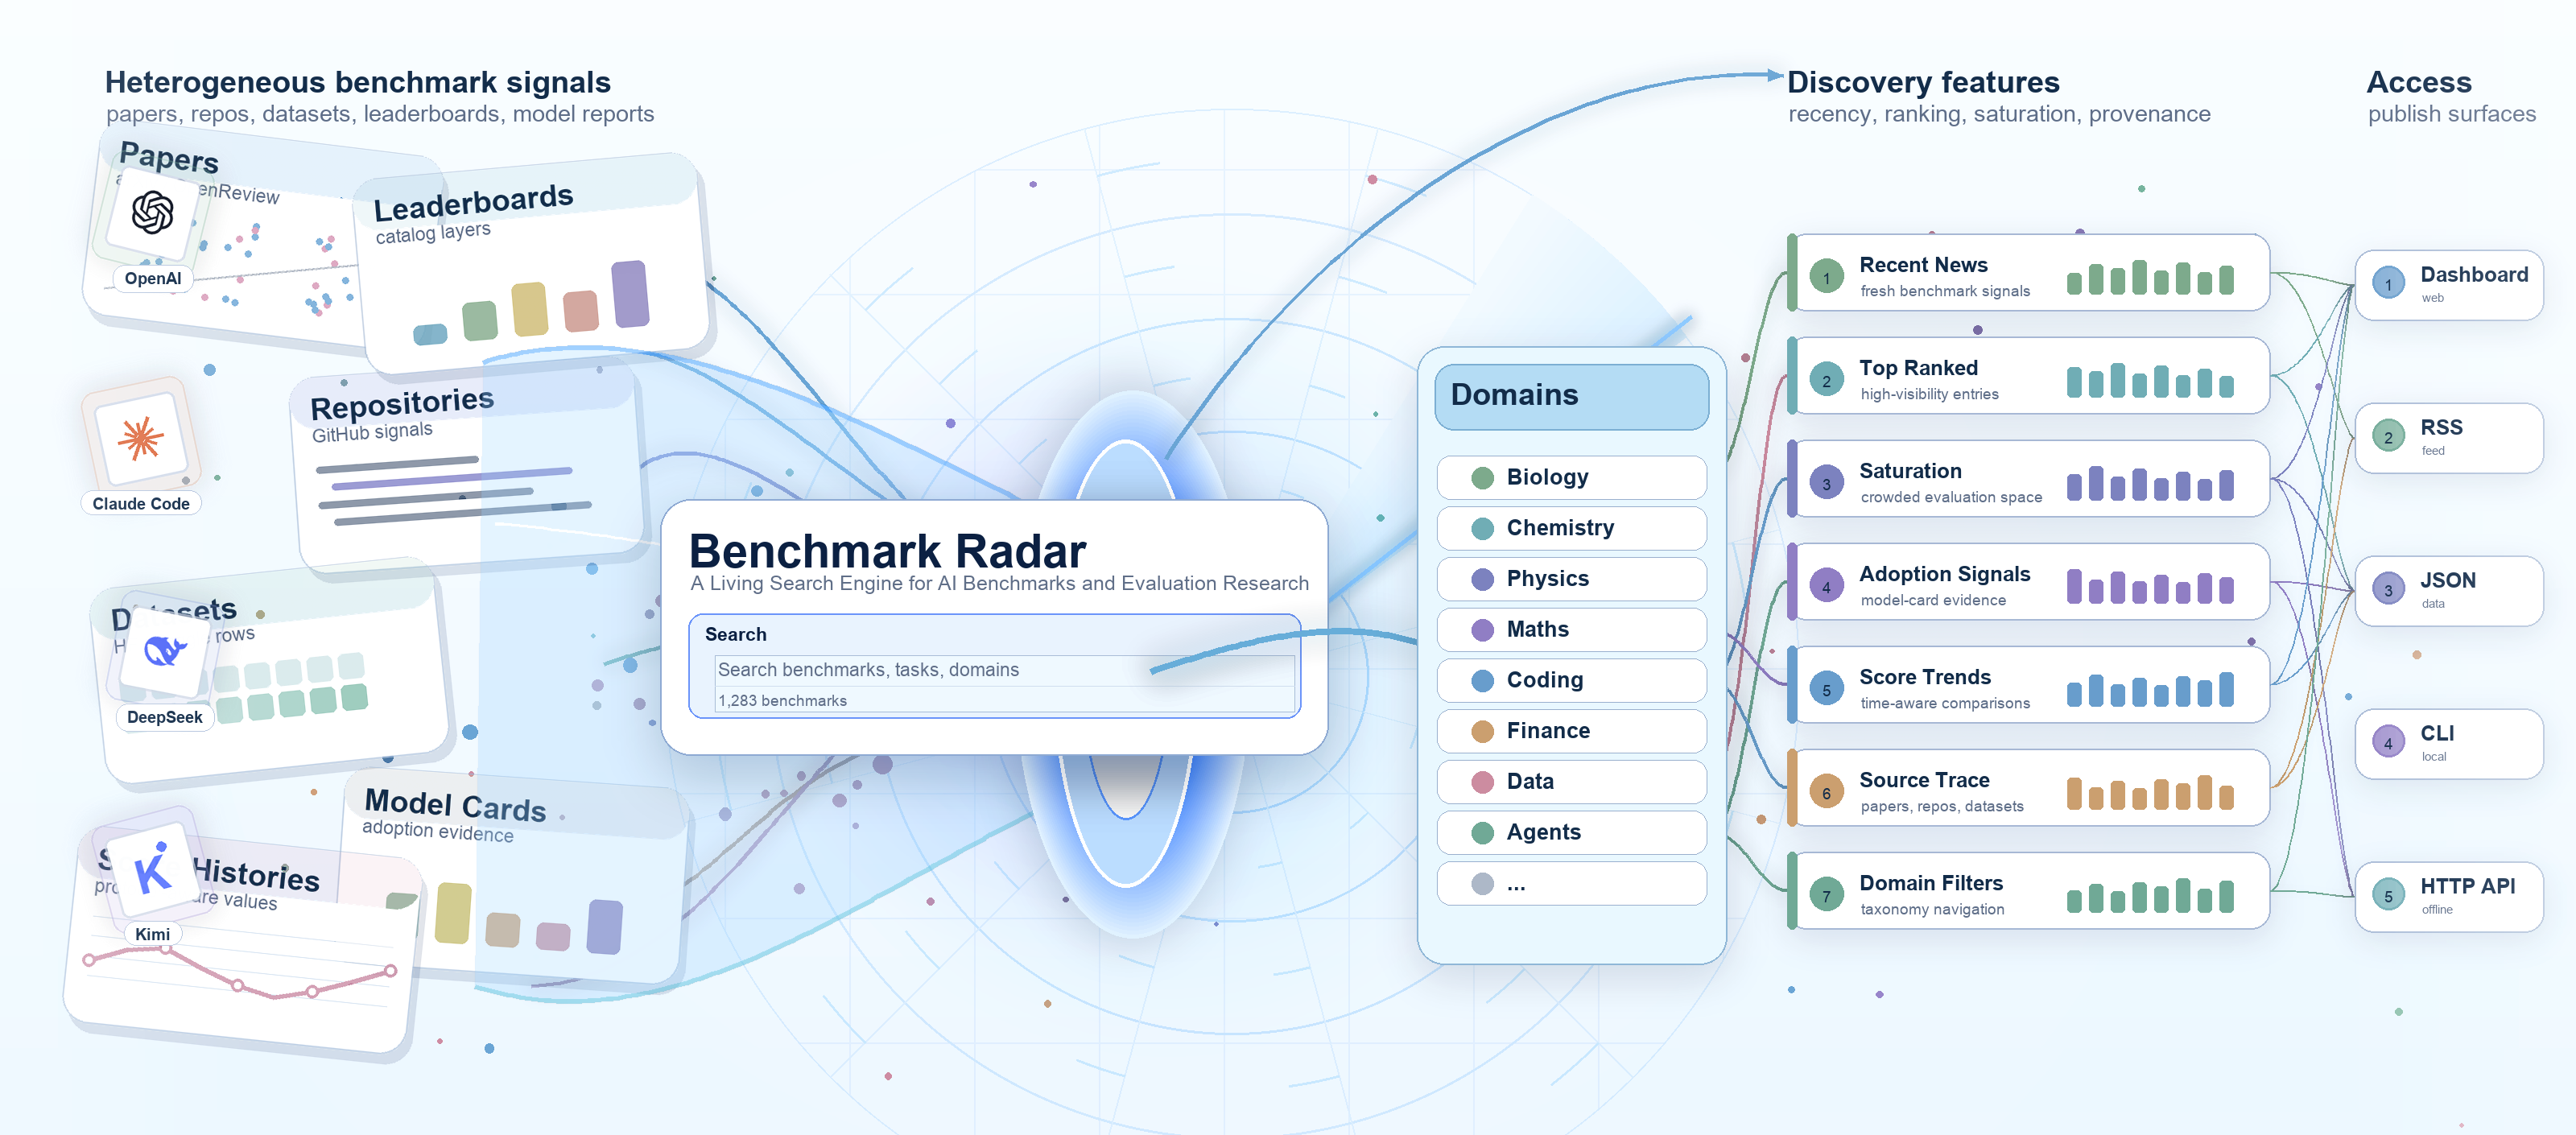
\includegraphics[width=0.92\textwidth,height=0.31\textheight]{abstract_overview.png}
\captionof{figure}{Benchmark Radar collects papers, repositories, datasets, and model reports, organizes them by topic, and makes them searchable alongside benchmark mentions and reported scores.}
\label{fig:abstract}
\vspace{0.8em}
\end{center}


\section{Introduction}

The Transformer architecture established attention-based sequence modeling as a foundation for modern large language models (LLMs) \citep{vaswani2017attention}. GPT-6 Astra and Claude Fable 5.1 are designed for coding, research, and tasks that span multiple tools \citep{openai2026gpt6astra,anthropic2026fable51}. Comparing these models requires benchmarks that expose failures and distinguish capability gains from changes in prompts, data splits, or evaluation procedures \citep{hendrycks2021mmlu,rein2023gpqa,phan2025hle,shang2026llm}.

Evaluation also matters beyond general-purpose chat. In recommender systems, Transformer-style sequence models and LLM-based methods support user, item, and preference modeling, with efficient training needed at production scale \citep{kang2018selfattentive,sun2019bert4rec,shang2026erase}. Foundation models are also used to model biological, geoscientific, and physical processes \citep{theodoris2023transfer,cui2024scgpt,shang2025predicting,zhang2025genetic,wu2023perturbations}. In social and political analysis, language models support text annotation and simulated human samples, while network methods quantify balance and polarization dynamics \citep{leskovec2010signed,gilardi2023chatgpt,argyle2023out,li2026matraix,ng2026microverse,shang2026inference}. Benchmark scores inform claims of progress across these scientific, industrial, and decision-support settings.

Benchmarks differ in the abilities they test. Broad evaluations of knowledge and reasoning include MMLU \citep{hendrycks2021mmlu}, GPQA \citep{rein2023gpqa}, and Humanity's Last Exam \citep{phan2025hle,zhou2026asi}. Others isolate more specific capabilities: SWE-bench measures whether models can resolve real GitHub issues \citep{jimenez2023swebench}, LiveCodeBench tests code generation with date-based splits to reduce contamination from training data \citep{jain2024livecodebench}, and Terminal-Bench and Long-Horizon-Terminal-Bench test command-line agents on operational tasks \citep{merrill2026terminalbench,li2026long}. Domain-specific evaluations include FinanceBench for finance and economics \citep{islam2023financebench}, MATH for mathematics \citep{hendrycks2021math}, SciBench for scientific problem solving \citep{wang2023scibench,wu2026esm,xu2026researchclawbench}, LAB-Bench for biology \citep{laurent2024labbench}, and ChemBench for chemistry \citep{mirza2025chembench}. Their tasks and scoring rules specify which model behaviors count as successful performance.

Finding a benchmark, its dataset or repository, and reports of its use requires searching paper servers, code hosting sites, dataset hubs, vendor releases, blogs, and benchmark catalogs. Existing resources such as LLM Stats, OpenCompass, and Artificial Analysis provide leaderboards, evaluation platforms, and model-analysis views \citep{llmstats2026benchmarks,opencompass2026datasetstatistics,artificialanalysis2026methodology}. To our knowledge, no existing system centers on benchmark search while combining daily discovery, catalog records, mentions in model reports, and scores with documented evaluation settings and sources.

Benchmark Radar gathers benchmark-related artifacts from public sources, groups observations with matching identifiers, and exposes a searchable index with source labels, dates, benchmark mentions, and scores. We present the search system, describe the collection and ranking methods needed to reproduce its outputs, and examine benchmark coverage, adoption in model reports, source concentration, and gaps in evaluation settings.\footnote{Source code: \url{https://github.com/ktwu01/benchmark-radar}.}

\section{Methodology}

\subsection{System Overview}

Benchmark Radar adapts the daily collection approach of BuilderPulse, which answers a fixed question set from more than ten sources each morning \citep{builderpulse}. It applies this approach to benchmark discovery, catalog search, and score histories. Readers can look for recent releases, search for a task or benchmark name, inspect mentions in model reports, and compare scores collected under matching evaluation settings. Table~\ref{tab:reader-questions} lists these uses and the interfaces that support them.

\begin{table}[htbp]
\centering
\small
\begin{tabularx}{\textwidth}{L{0.18\textwidth}Y Y}
\toprule
\textbf{Interface} & \textbf{Reader question} & \textbf{Role in Benchmark Radar}\\
\midrule
Today & What appeared or changed? & Ranks new records and links the source evidence.\\
Search box & Which records match this name, task, or domain? & Matches names, phrases, and query words in the benchmark index.\\
Leaderboard & Which benchmarks do labs report? & Counts benchmark mentions across curated model-card documents.\\
Scores & Which reported scores can be compared? & Groups scores by benchmark version, metric, and evaluation settings.\\
Trends and map & Which topics and sources recur? & Records source coverage so changes in collection can be considered when comparing topics.\\
CLI and HTTP & Can an analyst reproduce search locally? & Use one query service and a shared JSON response format.\\
\bottomrule
\end{tabularx}
\caption{Reader questions and the interfaces used to answer them.}
\label{tab:reader-questions}
\end{table}

The source systems expose different fields and identifiers. Benchmark Radar converts their records into common fields for names, descriptions, source labels, identifiers, dates, and supporting documents. A source observation is a collected record; an artifact is a paper, repository, dataset, release, or page identified from those observations. The benchmark catalog retains one record per benchmark within each source, so similarly named entries from different sources remain distinct. Model reports describe model development and evaluation, and their benchmark mentions provide evidence of adoption \citep{mitchell2019modelcards}. Here, adoption means a documented mention; it does not imply a comparable numeric score.

\subsection{Collection and Source Health}

Connectors are programs that retrieve records from public sources. Each collection run searches a 48-hour window, records counts and errors by source, removes future-dated rows, and requires healthy responses from a configured set of core sources before publication. The core sources at the cutoff were arXiv \citep{arxivapi}, Hugging Face Hub \citep{huggingfacehub}, and GitHub Search \citep{githubsearchdocs}. Optional routes include GitHub organizations, Hugging Face Papers, Kaggle datasets \citep{kaggleapi}, Zenodo \citep{zenodoapi}, OpenReview \citep{openreview}, Semantic Scholar \citep{kinney2023semanticscholar}, GitHub Releases \citep{githubreleasesdocs}, OpenAlex \citep{priem2022openalex}, Brave Search \citep{bravesearchapi}, 24 institution-operated research or engineering feeds, and a separate collector of public attention through Hacker News search on Algolia \citep{hnalgoliaapi}. All three core sources were healthy at the cutoff. Semantic Scholar was rate-limited, Brave Search lacked an API key, and OpenReview returned no eligible rows. Appendix~\ref{app:source-inventory} lists the healthy connectors and monitored feeds.

The collection run at the cutoff fetched 867 rows, reduced them to 837 candidate records after removing duplicates, classified 322 as eligible, and recommended 110 for readers to review. Two collections ran within the cutoff window; after merging, the daily page contained 322 records, including 110 recommendations. Published records retain the source URL, retrieval time, parser version, source identifier, timestamps, authors or organizations when supplied, and a SHA-256 checksum for verifying the stored record. Raw responses and credentials are excluded.

\begin{figure}[htbp]
\centering
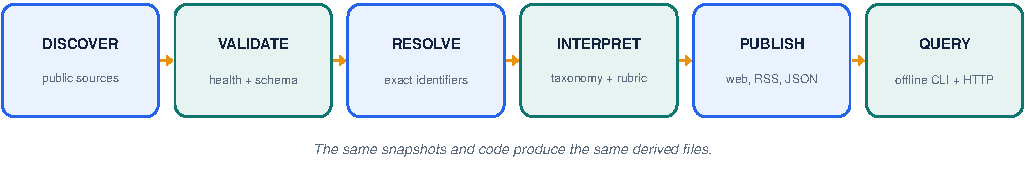
\includegraphics[width=\textwidth]{pipeline-evaluation.pdf}
\caption{Collection and publication stages. Connectors retrieve public records and check source health and record formats. Matching DOI, arXiv, OpenReview, GitHub, or Hugging Face identifiers link observations to artifacts. Classification and priority scoring organize the records before publication. Web pages, feeds, and local clients expose the collected evidence.}
\label{fig:pipeline}
\end{figure}

Dated snapshots, record formats, parser versions, and checksums allow the published data to be rebuilt and checked. Publication requires healthy core sources; failures in optional sources remain visible. Installed clients validate an update before activating it. Identity resolution relies on exact identifiers and reviewed links between source records. The evaluated release passed 1,236 tests after a clean rebuild. Section~\ref{sec:caveat-future-work} describes the remaining limitations.

\subsection{Identity, Ranking, and Search}

The resolver groups observations when they share a DOI, arXiv identifier, OpenReview identifier, GitHub repository, or Hugging Face artifact. Similar titles alone do not force a merge; they remain separate until review confirms that they describe the same artifact. This policy reduces false joins but leaves possible duplicates visible when papers, repositories, and catalogs lack a common identifier.

Search covers four catalog sources, as summarized in Table~\ref{tab:search-layers}: LLM Stats, OpenCompass Hub, Artificial Analysis, and Model reports. The index contains \ReportNumber{\ReportCatalogCount} source records, including \ReportModelReportCount{} model-report benchmarks. Of these model-report benchmarks, 86 have reported scores and 24 have no scores; both groups remain searchable. Search matches query words and phrases against record fields, including benchmark names. It searches all four sources together and preserves each result's source label. The same query against the same index produces the same ranking.

A separate priority score for daily recommendations combines relevance (35\%), evidence (20\%), recency (20\%), and adoption (25\%) on a 0--100 scale. These weights describe daily reading priority; search relevance depends on the query. The scoring configuration is included with the published data.

\begin{table}[htbp]
\centering
\small
\begin{tabularx}{\textwidth}{L{0.20\textwidth}rY}
\toprule
\textbf{Catalog source} & \textbf{Rows} & \textbf{Primary use}\\
\midrule
LLM Stats & \ReportLLMStatsCount{} & Benchmark names and descriptions with source provenance.\\
OpenCompass Hub & \ReportOpenCompassCount{} & Paper, repository, release, and dataset links with source-specific identity fields.\\
Artificial Analysis & \ReportArtificialAnalysisCount{} & Current commercial evaluation catalog entries.\\
Model reports & \ReportModelReportCount{} & Benchmarks mentioned in model reports, including records without scores.\\
Total & \ReportNumber{\ReportCatalogCount} & All four sources, retaining each record's source label.\\
\bottomrule
\end{tabularx}
\caption{Catalog sources in the Benchmark Radar query index.}
\label{tab:search-layers}
\end{table}

\subsection{Adoption and Score Curation}

Benchmark Radar records benchmark mentions and numeric scores from model-card and system-description documents \citep{mitchell2019modelcards}. This collection includes 37 model documents from 12 organizations. They mention 110 benchmarks whose names have been reconciled within the model-report collection. When a document contains an interpretable numeric value and sufficient context, the score archive records the benchmark version and metric (the instrument), along with evaluation settings (the protocol). These settings include examples supplied in the prompt (shots), tool access, attempts, and the evaluator when available. The archive contains 322 scores across 86 benchmark tracks. A score track groups results for a named benchmark; comparisons within it still require matching instruments and protocols. Scores from benchmark registries remain outside these model-report score histories unless they can be connected to a comparable protocol \citep{gebru2021datasheets,mitchell2019modelcards}.

\section{Results}
\label{sec:results}

\subsection{Coverage at the Cutoff}

At the \datacutoff{} cutoff, the cumulative discovery collection held \ReportNumber{\ReportObservationCount} source observations and \ReportNumber{\ReportArtifactCount} artifacts grouped by exact identifiers. Primary or structured sources supplied 10,473 observations, or 97.86\% of the collection. This category covers scholarly records, institution-operated feeds, code repositories, and dataset or artifact hosts. Discovery observations, benchmark records, model-report mentions, and scores count different objects and must not be added together. Table~\ref{tab:counts} defines each unit.

\begin{figure}[htbp]
\centering
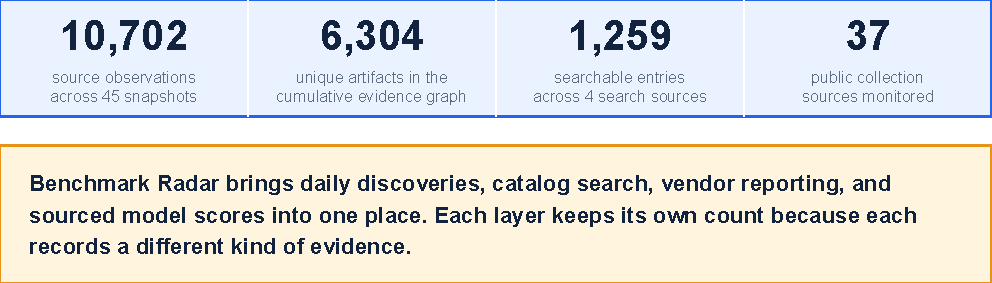
\includegraphics[width=0.96\textwidth]{cover-metrics.pdf}
\caption{Source observations, resolved artifacts, searchable benchmark records, and catalog sources as of \datacutoff{}.}
\label{fig:cover-metrics}
\end{figure}

\begin{table}[htbp]
\centering
\small
\begin{tabularx}{\textwidth}{L{0.24\textwidth}rY}
\toprule
\textbf{Unit} & \textbf{Count} & \textbf{Interpretation}\\
\midrule
Snapshot & \ReportSnapshotCount{} & Dated collection records, including 41 observed and 4 simulated snapshots.\\
Source observation & \ReportNumber{\ReportObservationCount} & Collected records with their source and retrieval information.\\
Unique artifact & \ReportNumber{\ReportArtifactCount} & Papers, repositories, datasets, releases, or pages grouped by matching identifiers.\\
Searchable entry & \ReportNumber{\ReportCatalogCount} & One benchmark record per source, including records without scores.\\
Adoption benchmark & 110 & Benchmarks mentioned in model reports, with names reconciled within that collection.\\
Model-card document & 37 & Curated reports from 12 organizations.\\
Curated score & 322 & Numeric results across 86 benchmark tracks.\\
\bottomrule
\end{tabularx}
\caption{What each count measures at \datacutoff{}.}
\label{tab:counts}
\end{table}

\subsection{Source Composition and Reliability}

Five source labels account for 9,532 of \ReportNumber{\ReportObservationCount} observations, or 89.1\% of the cumulative collection. Because these sources supply most observations, their retrieval caps, rate limits, and availability can change the apparent topic mix. At the cutoff, the required sources were healthy, while optional routes varied in yield because of rate limits, missing credentials, or empty result windows.

\begin{figure}[htbp]
\centering
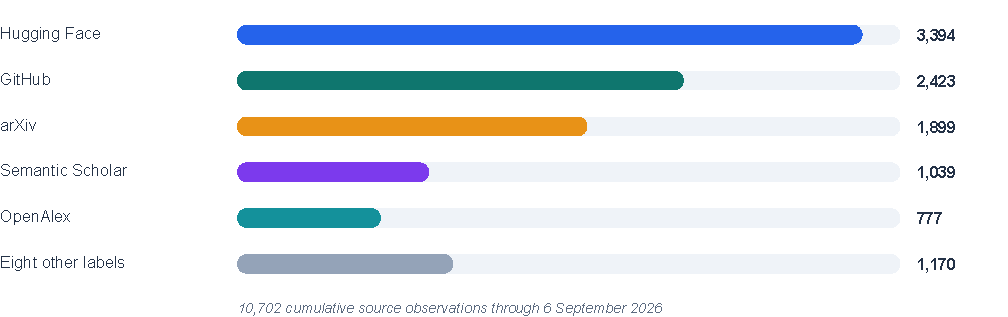
\includegraphics[width=0.92\textwidth]{source-composition.pdf}
\caption{Discovery observations by source through \datacutoff{}. The bars count collected observations, including repeat sightings, rather than distinct benchmarks.}
\label{fig:source-composition}
\end{figure}

Fifty-nine of \ReportNumber{\ReportArtifactCount} artifacts were linked across more than one source, or 0.94\% of the artifact set. Matching exact identifiers reduces false joins; links between papers, code, and datasets still require review when identifiers are missing or inconsistent.

\subsection{Relationship to Existing Catalogs}

Benchmark Radar imports records from three benchmark registries: LLM Stats, OpenCompass Hub, and Artificial Analysis. These projects have different goals. LLM Stats publishes live benchmark rankings and benchmark-family pages \citep{llmstats2026benchmarks}; OpenCompass is primarily an evaluation platform with a searchable dataset-statistics page \citep{opencompass2026datasetstatistics}; and Artificial Analysis publishes model evaluations and a documented intelligence-benchmarking methodology \citep{artificialanalysis2026methodology}.

The index contains \ReportLLMStatsCount{} records from LLM Stats, \ReportOpenCompassCount{} from OpenCompass Hub, \ReportArtificialAnalysisCount{} from Artificial Analysis, and \ReportModelReportCount{} from Model reports, yielding \ReportNumber{\ReportCatalogCount} searchable source records. Records without scores remain in this total; source membership does not establish a trust ranking. Direct comparisons of totals would be misleading because record definitions, update frequency, source coverage, and evaluation settings differ across systems. Benchmark Radar combines these catalog records with daily discovery, artifact links based on matching identifiers, mentions in model reports, and scores with documented evaluation settings.

\subsection{Benchmark Adoption in Model Reports}

In the model-report collection, eight benchmarks appeared in documents from at least six organizations: GPQA Diamond \citep{rein2023gpqa}, Humanity's Last Exam \citep{phan2025hle}, SWE-bench Verified \citep{jimenez2023swebench}, Terminal-Bench \citep{merrill2026terminalbench}, AIME \citep{maa2026aime}, LiveCodeBench \citep{jain2024livecodebench}, MMLU-Pro \citep{wang2024mmlupro}, and BrowseComp \citep{wei2025browsecomp}. GPQA Diamond appeared in 27 of 37 documents from 11 organizations, making it the most commonly mentioned benchmark in these reports. This concentration suggests that frontier-model reporting has partly converged on a common set of evaluations, even as researchers introduce benchmarks in other areas.

A benchmark can be widely mentioned without providing comparable scores across dates. Comparing scores can be misleading when reasoning budget, tool access, attempts, evaluator, or date-based test split differs \citep{gebru2021datasheets,mitchell2019modelcards}. A near-ceiling result applies to the reported evaluation setup; it does not by itself establish benchmark saturation.

\section{Limitations and Future Work}
\label{sec:caveat-future-work}

Lexical search can miss paraphrased benchmark names, renamed tasks, or descriptions of related ideas. Optional semantic retrieval could find such records by meaning, while retaining the source, field, and word matches that let readers inspect each result \citep{reimers2019sentencebert}. Source coverage also depends on public endpoints, API credentials, and rate limits. Counts need units and a data cutoff so readers can distinguish changes in collection from changes in benchmark activity.

Exact identifiers reduce false joins but leave possible links between papers, code, and datasets unresolved when identifiers are absent. Further identity review should link repositories to papers and document the evidence for each decision. In the snapshot, 12,594 scores from benchmark registries remain outside the model-report score histories because they lack protocol fields such as prompt examples, tool access, attempts, evaluator, date-based test splits, or evaluation software. Recording these settings would allow more scores to be compared.

Task-level coverage is also incomplete. The capability-classification component, KW-Bench, has 5,661 tracks without complete task-capability labels at the cutoff. Here, a classification track is an artifact or a declared task within a benchmark suite, drawn from discovery observations; it is a different unit from a catalog record or a model-report score track. These missing labels limit conclusions about which abilities the collected tasks test. Completing them would help readers identify the capability a task requires. Counts in the dashboard and local outputs also need consistent labels for observations, artifacts, benchmark records, mentions, and scores.

\section{Conclusion}

Benchmark Radar brings benchmark discovery, catalog search, model-report mentions, and score histories into one system while retaining the sources behind each record. The evaluated snapshot combines 37 public source routes, a \ReportNumber{\ReportCatalogCount}-record search index, and adoption evidence from 37 model documents.

Readers can use this evidence to find candidate benchmarks and inspect their reporting history. Comparing scores still requires checking the benchmark version and evaluation settings. Missing identifiers leave some artifact relationships unresolved, and missing protocol details prevent many scores from supporting comparisons across dates.

\begingroup
\small
\raggedright
\bibliographystyle{plainnat}
\bibliography{references}
\endgroup

\clearpage
\appendix
\begin{center}
{\LARGE\bfseries Appendix}
\end{center}
\vspace{0.75em}

\section{Source Inventory and Health}
\label{app:source-inventory}

Table~\ref{tab:healthy-connectors} lists source connectors that completed successfully at the cutoff. Row counts are measured before duplicate removal and ranking. A connector can be healthy with zero eligible rows if its request succeeds and the response can be parsed. Core sources cover papers, shared model or dataset artifacts, and code; all must be healthy before publication. Failures in optional sources are reported but do not block publication.

\begin{center}
\begin{minipage}{\textwidth}
\centering
\small
\begin{tabularx}{\textwidth}{L{0.21\textwidth}Y L{0.21\textwidth}L{0.08\textwidth}}
\toprule
\textbf{Connector} & \textbf{Role} & \textbf{Cutoff status} & \textbf{Core}\\
\midrule
arXiv & Primary papers via selected AI, language, vision, and software categories & Healthy; 0 rows & Yes\\
Hugging Face Hub & Datasets and Spaces connected to benchmark artifacts & Healthy; 92 rows & Yes\\
GitHub Search & Code repositories and benchmark artifacts & Healthy; 300 rows; at cap & Yes\\
GitHub Organizations & Reviewed organization repositories & Healthy; 4 rows & No\\
Hugging Face Papers & Community-surfaced papers & Healthy; 0 rows & No\\
Kaggle Datasets & Public benchmark datasets & Healthy; 32 rows & No\\
Zenodo & DOI-bearing research artifacts & Healthy; 57 rows & No\\
OpenReview & Conference submissions & Healthy; no eligible rows & No\\
GitHub Releases & Curated first-party releases & Healthy; 6 rows & No\\
OpenAlex & Scholarly discovery metadata & Healthy; 200 rows & No\\
\bottomrule
\end{tabularx}
\captionof{table}{Healthy direct discovery connectors at the current cutoff.}
\label{tab:healthy-connectors}
\end{minipage}
\end{center}

Table~\ref{tab:first-party-feeds} lists research and engineering feeds operated by the institutions being monitored. They can surface benchmark papers, datasets, model announcements, and engineering posts. The feed collector yielded one relevant record at the cutoff. Some healthy feeds produced zero matches after relevance filtering. Searches restricted to an organization's website cover institutions that lack a verified feed.

\begin{center}
\begin{minipage}{\textwidth}
\centering
\small
\begin{tabularx}{\textwidth}{Y Y}
\toprule
\textbf{Feeds 1-12} & \textbf{Feeds 13-24}\\
\midrule
Meituan Engineering & Ai2\\
OpenAI News & Together AI\\
Google AI & Sakana AI\\
Google DeepMind & Qwen\\
Google Research & Ollama\\
Apple Machine Learning Research & Stability AI\\
AWS Machine Learning & Nomic AI\\
Hugging Face Blog & Replicate\\
Microsoft Research & NVIDIA Developer\\
NVIDIA AI Blog & IBM Research\\
Mistral AI & Databricks\\
Meta Research & LangChain\\
\bottomrule
\end{tabularx}
\captionof{table}{First-party research and engineering feeds monitored by Benchmark Radar.}
\label{tab:first-party-feeds}
\end{minipage}
\end{center}

\section{Worked Use Case: Prior-Art Check for a New Evaluation}
\label{app:use-case}

This case describes one contributor's use of Benchmark Radar to check related work before designing an evaluation. It is a single workflow, with no measured timing or accuracy outcome.

The contributor wanted to determine whether a proposed evaluation duplicated existing work. The session ran during August 2026 and surveyed recent work on credit assignment in agentic training, using small Qwen-series models as a requirement for reproducible baseline experiments. Comparing a candidate design against existing work normally requires manual searches, whose completeness is difficult to establish.

The contributor gave the task to a coding agent together with the public setup instructions for Benchmark Radar. The agent installed the command-line client and the Benchmark Radar Skill, a set of instructions for using the client. It then downloaded the local corpus and queried candidate records offline.

\begin{center}
\begin{minipage}{\textwidth}
\centering
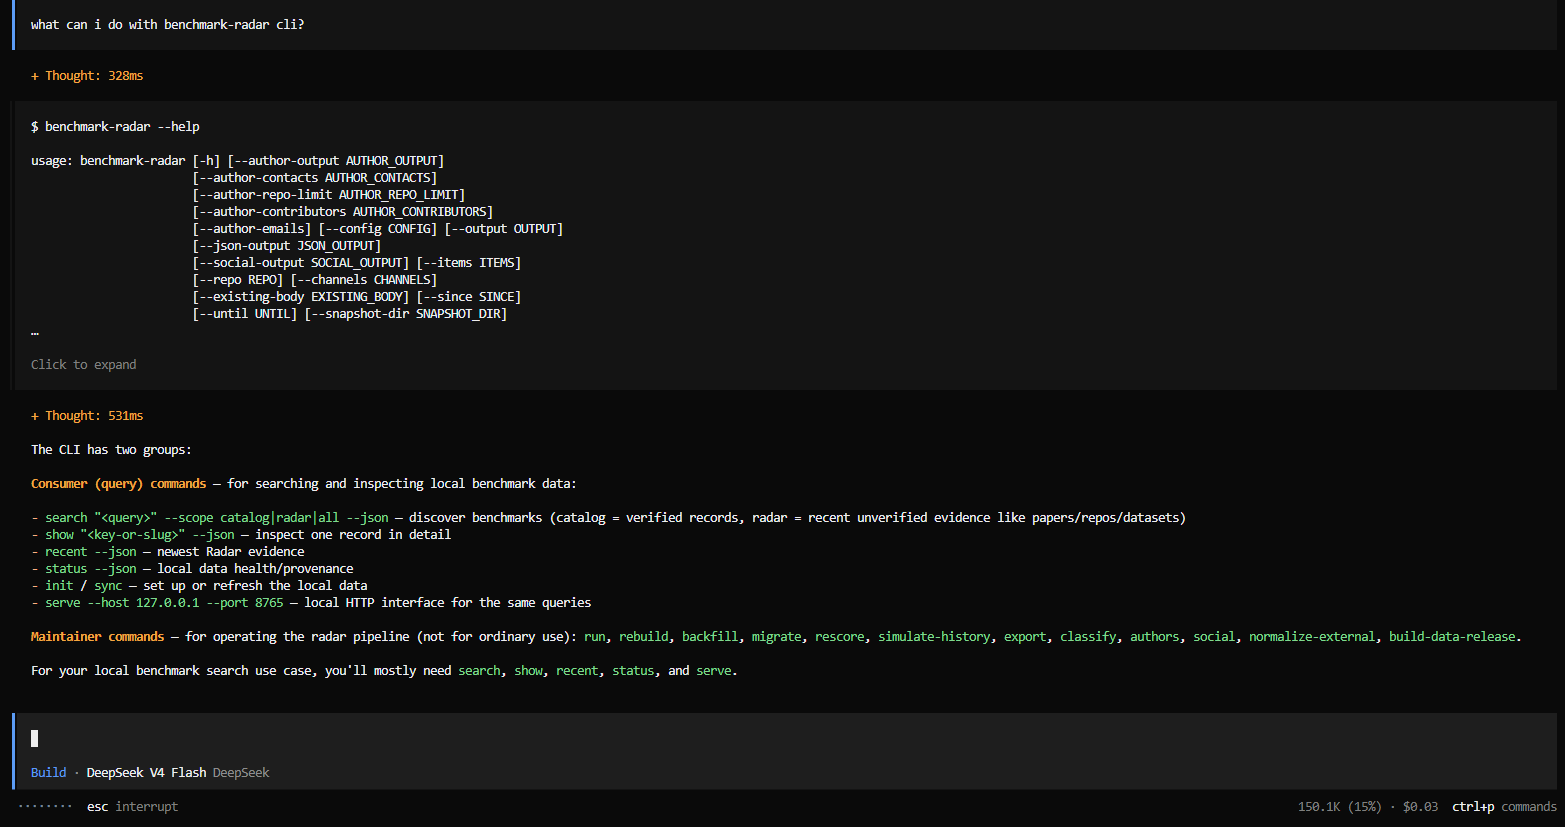
\includegraphics[width=0.92\textwidth]{agent-session.png}
\captionof{figure}{A coding agent installs the Benchmark Radar client and its usage instructions, then runs local queries.}
\label{fig:use-case-session}
\end{minipage}
\end{center}

The agent inspected which paper, repository, and dataset links were recorded for each candidate. Figures~\ref{fig:use-case-paper} and~\ref{fig:use-case-code} show records with a repository link and no dataset link. The paper-link field differs between them. A missing link describes the collected record; it does not establish that the artifact has not been released.

\begin{center}
\begin{minipage}{\textwidth}
\centering
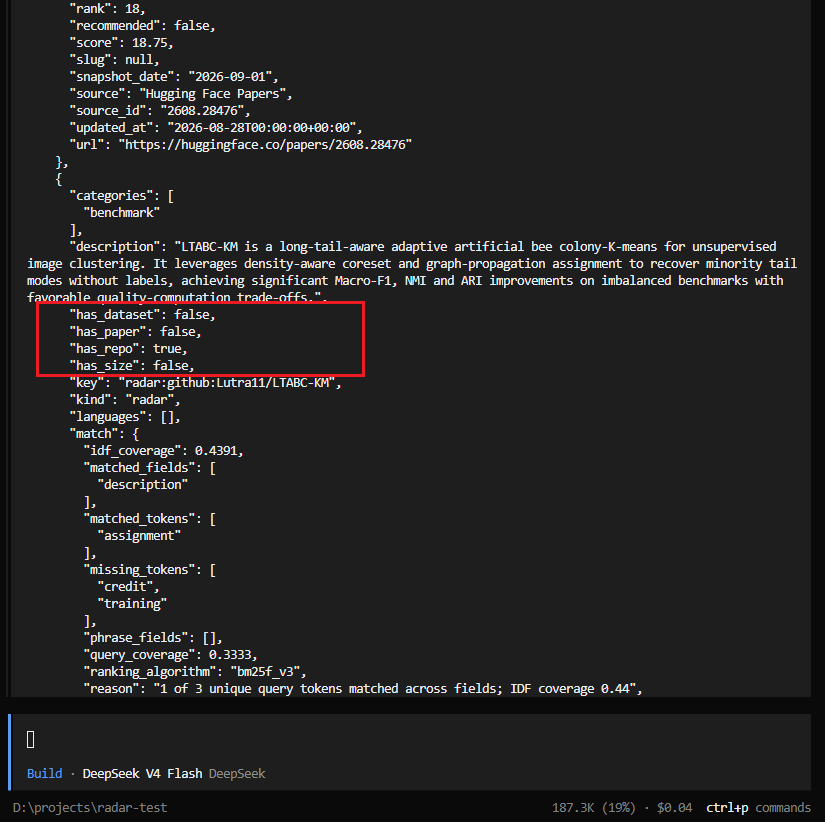
\includegraphics[width=0.92\textwidth]{artifact-status-paper.png}
\captionof{figure}{A retrieved record with a repository link, no dataset link, and a false paper-link field. These fields describe the links recorded by the client.}
\label{fig:use-case-paper}
\end{minipage}
\end{center}

\begin{center}
\begin{minipage}{\textwidth}
\centering
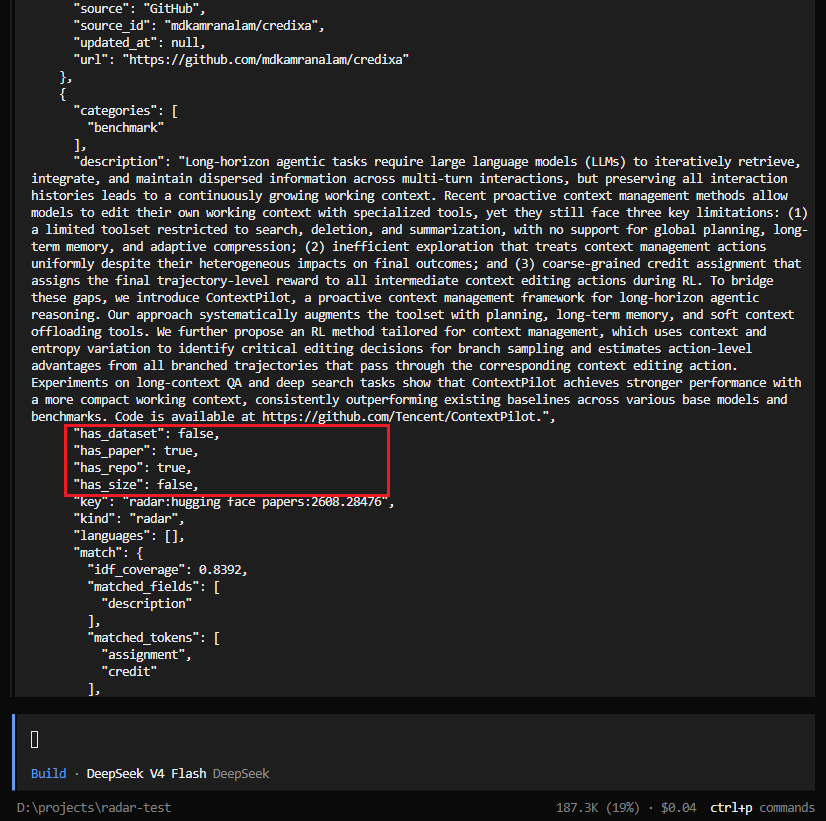
\includegraphics[width=0.92\textwidth]{artifact-status-code.png}
\captionof{figure}{A second retrieved record with paper and repository links but no dataset link. The missing dataset link does not establish its release status.}
\label{fig:use-case-code}
\end{minipage}
\end{center}

Benchmark Radar search matches words and phrases, so the agent also ran its own web search and cross-checked the two candidate sets before accepting a record. The additional search checked for related work described in different terms. The agent still had to judge whether each retrieved record was relevant to the proposed evaluation.

\begin{center}
\begin{minipage}{\textwidth}
\centering
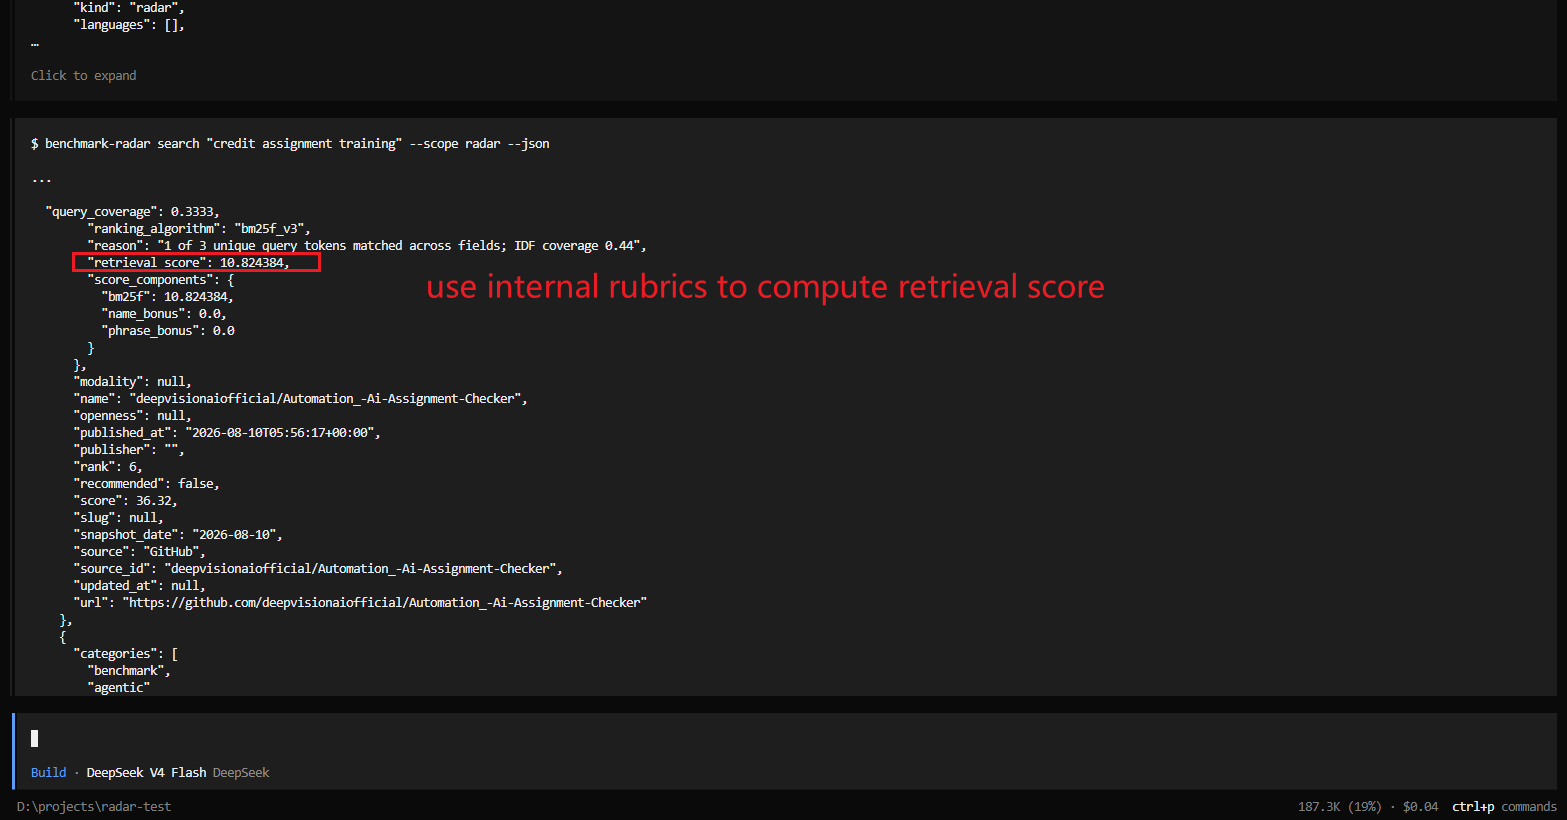
\includegraphics[width=0.92\textwidth]{cross-validation.png}
\captionof{figure}{A candidate record with query-word matches and retrieval-score components for the agent to inspect when judging relevance.}
\label{fig:use-case-cross}
\end{minipage}
\end{center}

The session ended with a focused summary table of related work that the contributor judged complete enough to act on.

\begin{center}
\begin{minipage}{\textwidth}
\centering
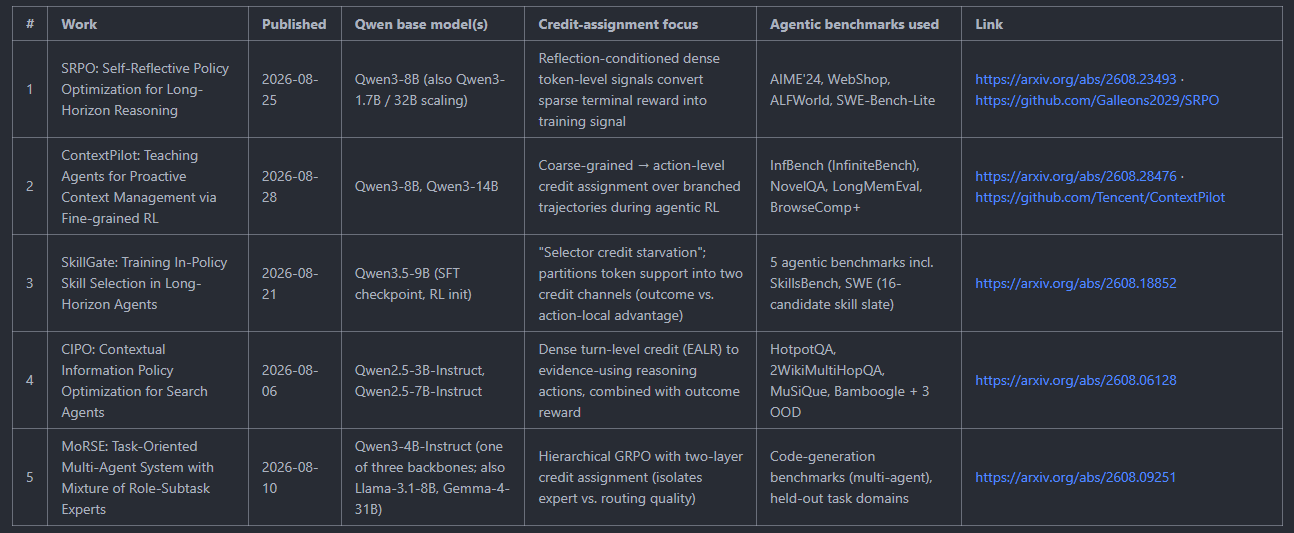
\includegraphics[width=0.92\textwidth]{survey-table.png}
\captionof{figure}{Summary table of recent work on credit assignment in agentic training, assembled during the session.}
\label{fig:use-case-survey}
\end{minipage}
\end{center}

Figure~\ref{fig:use-case-manual-table} shows a comparison table from an earlier benchmark-design effort by one contributor. It covers ten related benchmarks across six design dimensions, with each cell read from a source paper. The contributor reported that assembling it took more effort than any part of that project except producing the benchmark data. Benchmark Radar retrieves candidates for this kind of comparison and exposes the matching words and fields for inspection; the comparison itself requires reading the source evidence.

\begin{center}
\begin{minipage}{\textwidth}
\centering
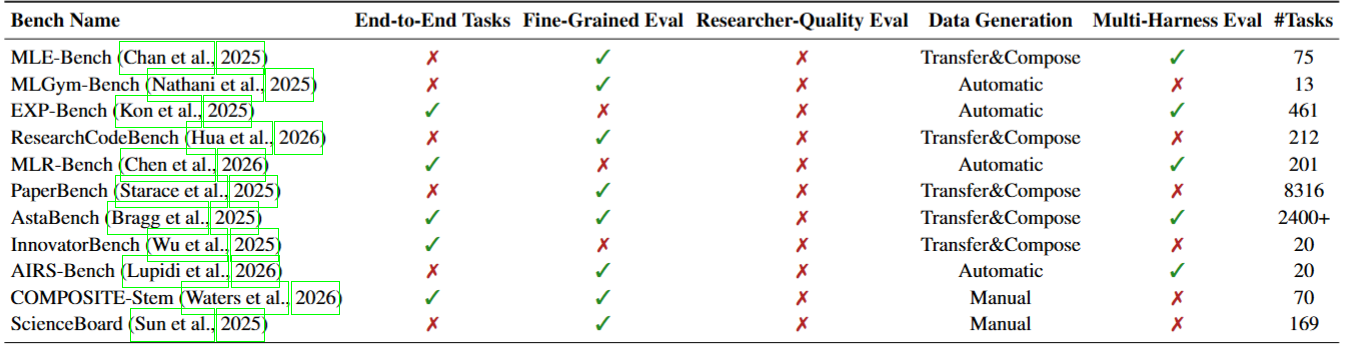
\includegraphics[width=0.98\textwidth]{manual-prior-art-table.png}
\captionof{figure}{A prior-art comparison table assembled manually for an earlier benchmark-design effort. Each row is one related benchmark and each column one design dimension, all read from the source papers by hand.}
\label{fig:use-case-manual-table}
\end{minipage}
\end{center}

Query wording can change the candidate set because search matches words rather than meaning. The session combined Benchmark Radar with the agent's web search, so it does not isolate either tool's contribution. Repository and dataset availability can also change after retrieval. The summary table and screenshots document one workflow, without a controlled comparison. Additional session evidence is available in the project's public \href{https://github.com/ktwu01/benchmark-radar/issues/492}{issue~\#492}.

\section{Contributor Credit}
\label{app:contributor-credit}

Junjie Zhou contributed a score-archive audit and earlier report revisions, documented in \href{https://github.com/ktwu01/benchmark-radar/issues/457}{issue~\#457}. Jiayu Wang contributed the worked use case in Appendix~\ref{app:use-case} and its supporting evidence, documented in \href{https://github.com/ktwu01/benchmark-radar/issues/492}{issue~\#492}.

\section{Reproducibility, Access, and Citation}
\label{app:reproducibility}

This paper evaluates Benchmark Radar \reportversion{} at Git commit \gitcommit{} with a data cutoff of \datacutoff{}. The data build combines dated collection snapshots, benchmark registry records, and model reports, then classifies tracks and packages the results with checksums. Installed clients validate the checksum and record format before activating an update. The evaluation used a clean data rebuild with linting, formatting checks, catalog normalization, classification, release construction, and the full test suite; all 1,236 tests passed. The manuscript is authored in LaTeX, separately from the data generators. The project provides a DOI and a Citation File Format record for citation \citep{smith2016,katz2021,cff}.

\begin{table}[htbp]
\centering
\small
\begin{tabularx}{\textwidth}{L{0.28\textwidth}Y}
\toprule
\textbf{Artifact} & \textbf{Canonical or permanent location}\\
\midrule
Archived paper (v0.9.0) & \url{https://doi.org/10.5281/zenodo.22167102}\\
Source code & \url{https://github.com/ktwu01/benchmark-radar}\\
Dashboard & \url{https://benchmark-radar.org/}\\
Discovery observations (JSON) & \url{https://benchmark-radar.org/data/radar.json}\\
Benchmark catalog & \url{https://benchmark-radar.org/data/benchmark-index.json}\\
RSS & \url{https://benchmark-radar.org/feed.xml}\\
Citation metadata & \url{https://github.com/ktwu01/benchmark-radar/blob/main/CITATION.cff}\\
\bottomrule
\end{tabularx}
\caption{Access and citation artifacts for Benchmark Radar.}
\label{tab:access-artifacts}
\end{table}

The reported counts were computed from the cumulative discovery data, benchmark catalog, model registry, model-report and score archives, normalized catalog records, and collection configuration. Their repository locations are \texttt{site/data/radar.json}, \texttt{site/data/benchmark-index.json}, \texttt{site/data/models.json}, \texttt{data/model\_cards.yml}, \texttt{data/benchmark\_scores.yml}, \texttt{data/catalog/}, and \texttt{config.yml}. The dated numerical inputs used by the manuscript and figures are stored in \texttt{figure-data.tex} beside the LaTeX source.

To reproduce the data build from a clean checkout, install the project and run \texttt{benchmark-radar normalize-catalog}, \texttt{benchmark-radar classify}, and \texttt{benchmark-radar build-data-release}, in that order. Run \texttt{make} in \texttt{docs/technical-report/latex/} to build this manuscript from its dated numerical inputs. Rebuilding the data at a later revision does not update those inputs automatically.

The DOI in Table~\ref{tab:access-artifacts} identifies the archived v0.9.0 paper. This manuscript describes \reportversion{} at the cutoff above. The dashboard continues to change; citations of its live counts need a retrieval date.

% \section{Licensing}
% Software: MIT License. The paper and original editorial content: CC BY-NC 4.0.
% Commercial republication, resale, paid newsletters, dataset packaging, or commercial
% product integration requires prior written permission from Koutian Wu. Third-party
% source material remains under its original terms.

\end{document}
